\documentclass[answers]{exam}
\usepackage{../../template}
\author{niceguy}
\title{Problem Set 4}
\begin{document}
\maketitle

\begin{questions}

\question{Consider a region with a uniform electrostatic field of intensity $E$. If the electric scalar potential at the point $A$ is zero, the potential at the point $B$ equals}

\begin{solution}
	$$V_B = -Ed\cos\alpha$$
\end{solution}

\question{A point charge $Q$ is situated in free space. The line integral of the electric field intensity vector $\vec{E}$ due to this charge along the contour $C$, composed of two circular parts of radii $a$ and $2a$, respectively, and two radial parts of length $a$, amounts to}

\begin{solution}
	$\vec{E}$ is conservative, so the integral is 0.
\end{solution}

\question{What happens to electric potentials and voltages in an electrostataic system after a new reference point is adopted for the potential?}

\begin{solution}
	Potentials change by the same value and voltages remain unchanged.
\end{solution}

\question{The electrostatic potential $V$ in a aregion is a function of the rectangular coordinate $x$ only. Consider the electric field intensities at points $A,B,C,D$, and $E$. The largest field intensity is at point}

\begin{solution}
	It is where the slope is maximum, which is $C$.
\end{solution}

\question{Consider an electrostatic field in a region of space and the following two statements. Which of the statements is true?}

\begin{parts}
	\part{If the electric scalar potential at a point in the region is zero, then the electric field vector at that point must be zero as well.}
	\part{If the electric field vector at a point in zero, then the potential at the same point must be zero.}
\end{parts}

\begin{solution}
	None of the statements are true. The statements simply discuss if there is any implication between $x=0$ and $x'=0$, where obvious counterexamples can be found.
\end{solution}

\question{An uncharged thin metallic rod is introduced into a uniform electrostatic field, of intensity vector $\vec{E}_0$, in free space, such that it is either perpendicular or parallel to $\vec{E}_0$. The rod affects the original field}

\begin{solution}
	Less in case (a). As the rod is a conductor, the electric field becomes close to zero, depending on conductivity.
\end{solution}

\question{A uniform electric field, of intensity vector $\vec{E}_0$, is established in the air-filled space between two metallic electrodes. If an uncharged (thick) metallic slab is then inserted in this space, without touching the electrodes, the electric field intensity vector in region 3 in the new electrostatic state is}

\begin{solution}
	$$E = \frac{V}{d}$$
	where $d$ is the distance. Substituting $V$ with $\frac{V}{2}$ and $d$ with $\frac{d}{3}$ gives
	$$\vec{E}_3 = \frac{3\vec{E}_0}{2}$$
\end{solution}

\question{A negatively charged small body is situated inside an uncharged spherical metallic shell. The distribution of induced charges on the outer surface of the shell can be represented as in}

\begin{solution}
	A
\end{solution}

\question{In order to protect body $B$ from the electrostatic field due to a charged body $A$, an ungrounded closed metallic screen is introduced. The protection is achieved for}

\begin{solution}
	b only.
\end{solution}

\question{point charge $Q$ is situated in air at a height $h$ above a grounded conducting plane. Relative to the plane, the electric force on this charge is}

\begin{solution}
	Always attractive.
\end{solution}

\question{The electrostatic potential $V$ in a region is a function of a single rectangular coordinate $x$, $V(x)$ and is shown in the figure below. Sketch the components of the electric field intensity $E$ in this region}

\begin{solution}
	\begin{tabular}{|c|c|c|c|c|c|c|c|c|c|c|}
		\hline
		$x$ & 0-1 & 1-2 & 2-3 & 3-4 & 4-5 & 5-6 & 6-7 & 7-8 & 8-9 & 9-10 \\
		\hline
		$E(x)$ & 2 & 1 & 0 & -1 & -2 & -2 & -1 & 0 & 1 & 2 \\
		\hline
	\end{tabular}
\end{solution}

\question{For the three charges in the figure below, calculate the electric potential at points defined by}

\begin{parts}
	\part{(0,0,2)}
	\part{(1,1,1)}
\end{parts}

\begin{solution}
	$(0,0,2)$:
	$$\frac{2\times10^{-6}k}{1} - \frac{2\times10^{-6}k}{\sqrt{5}} + \frac{10^{-6}k}{\sqrt{5}} = 10^{-6}k\left(2-\frac{1}{\sqrt{5}}\right)$$
	$(1,1,1)$:
	$$\frac{(1-2+2)10^{-6}k}{\sqrt{2}} = \frac{10^{-6}k}{\sqrt{2}}$$
\end{solution}

\question{For the semi-circular line charge in the figure below, the electric field at an arbitrary point on the $z$-axis has an $x$ and a $z$ component (confirm). Find the $z$-component of the field from the potential $V(0,0,z)$. Can you find the $x$-component too using $V (0,0,z)$?}\label{q}

\begin{solution}
	By symmetry, there is no $y$ component.
	\begin{align*}
		V(0,0,z) &= \int \frac{kdQ}{r} \\
			 &= \int_{-\frac{\pi}{2}}^\frac{\pi}{2} \frac{ka\rho_ld\phi}{\sqrt{a^2+z^2}} \\
			 &= \frac{ka\rho_l\pi}{\sqrt{a^2+z^2}} \\
			 &= \frac{kQ}{\sqrt{a^2+z^2}}
	\end{align*}
	Then the $z$-component is
	\begin{align*}
		E_z &= -\frac{dV(0,0,z)}{dz} \\
		    &= \frac{kQ}{2(a^2+z^2)^{3/2}} \times 2z \\
		    &= \frac{kQz}{(a^2+z^2)^{3/2}}
	\end{align*}
	The $x$-component cannot be found.
\end{solution}

\question{Two point charges $Q_1 = 7\unit{\mu.C}$, and $Q_2 = -3\unit{\mu.C}$, are located on two non-adjacent vertices of a square contour $a=15\unit{cm}$ on a side. Find the voltage between any of the remaining two vertices of the square and the square center.}

\begin{solution}
	By symmetry, both voltages are the same.
	$$\frac{(7-3)\times10^{-6}k}{0.15} - \frac{(7-3)\times10^{-6}k}{0.15\div\sqrt{2}} = -99.3\unit{kV}$$
\end{solution}

\question{Obtain the expression for the electric field intensity of a point charge at the origin from its potential.}

\begin{solution}
	Division by $r$.
\end{solution}

\question{Determine the work done in carrying a $-2\unit{\mu.C}$ charge from $P_1(2,1,-1)$, to $P_2(8,2,-1)$ in the field $\vec{E} = \hat{a}_xy + \hat{a}_yx$}

\begin{parts}
	\part{Along the parabola $x = 2y^2$}
	\part{Along the straight line joining $P_1$ and $P_2$}
\end{parts}

\begin{solution}
	\begin{align*}
		E &= -\int \vec{F}\cdot d\vec{l} \\
		  &= 2\times10^{-6} \int (\hat{a}_xy + \hat{a}_yx)\cdot d\vec{l}
	\end{align*}
	For the parabola,
	$$E = 2\times10^{-6} \int_1^2 (\hat{a}_xy + \hat{a}_y2y^2)\cdot (4y\hat{a}_x + \hat{a}_y)dy = 2\times10^{-6} \int_1^2 (4y^2 + 2y^2)dy = 28\times10^{-6}$$
	For the line,
	$$E = 2\times10^{-6} \int_1^2 (\hat{a}_xy + \hat{a}_y(6y-4)) \cdot (6\hat{a}_x + \hat{a}_y)dy = 2\times10^{-6} \int_1^2 (6y+6y-4)dy = 28\times10^{-6}$$
\end{solution}

\question{Three charges ($+q,-2q$, and $+q$) are arranged along the $z$-axis at $z = \frac{d}{2}, z = 0$, and $z = -\frac{d}{2}$, respectively.}

\begin{parts}
	\part{Determine $V$ and $\vec{E}$ at a distant point $P(R,\theta,\phi)$.}
	\part{Find the equations for equipotential surfaces and streamlines.}
	\part{Sketch a family of equipotential llines and streamlines.}
\end{parts}

\begin{solution}
	$$V = \frac{kQ}{r} = \frac{kq}{\sqrt{(R\cos\theta-\frac{d}{2})^2 + (R\sin\theta)^2}} - \frac{2kq}{R} + \frac{kq}{\sqrt{(R\cos\theta+\frac{d}{2})^2 + (R\sin\theta)^2}}$$
	Note that the denominator can be written as
	$$\sqrt{R^2\pm d\cos\theta R + \frac{d^2}{4}} = R\sqrt{1\pm \frac{d\cos\theta}{R} + \frac{d^2}{4R^2}}$$
	Approximating the square root,
	$$\left(1\pm\frac{d\cos\theta}{R}+\frac{d^2}{4R^2}\right)^{\frac{1}{2}} \approx 1 \mp \frac{d\cos\theta}{2R} - \frac{d^2}{8R^2} + \frac{3d^2\cos^2\theta}{8R^2} + \frac{3d^4}{128R^4} \pm \frac{3d^3\cos\theta}{16R^3} \approx 1 \mp \frac{d\cos\theta}{2R} - \frac{d^2}{8R^2} + \frac{3d^2\cos^2\theta}{8R^2}$$
	Then
$$V = \frac{kq}{R}\left(1 - \frac{d\cos\theta}{2R} - \frac{d^2}{8R^2} + \frac{3d^2\cos^2\theta}{8R^2} - 2 + 1 + \frac{d\cos\theta}{2R} - \frac{d^2}{8R^2} + \frac{3d^2\cos^2\theta}{8R^2}\right) = \frac{kqd^2}{4R^3}\left(3\cos^2\theta - 1\right)$$
	Note that due to symmetry, $\vec{E}$ has no $\hat{a}_\phi$ component.
	\begin{align*}
		\vec{E} &= -\vec{\nabla}V \\
			&= -\frac{\partial V}{\partial R}\hat{a}_R - \frac{1}{R}\frac{\partial V}{\partial \theta}\hat{a}_\theta \\
			&= \frac{3kqd^2}{4R^4}(3\cos^2\theta - 1)\hat{a}_R + \frac{kqd^2}{4R^4}(6\cos\theta\sin\theta)\hat{a}_\theta \\
			&= \frac{3kqd^2}{4R^4}((3\cos^2\theta - 1)\hat{a}_R + \sin2\theta\hat{a}_\theta) \\
	\end{align*}
\end{solution}

\question{Given the finite line charge $\rho_l$ of length $L$, find the potential on the cylindrical surface of radius $b$ as a function of $x$ and plot it.}

\begin{solution}
	\begin{align*}
		V(X) &= \int_0^L \frac{k\rho_l dx}{\sqrt{(x-X)^2+b^2}} \\
		     &= k\rho_l \int_{\arctan\left(-\frac{X}{b}\right)}^{\arctan\left(\frac{L-X}{b}\right)} \frac{b\sec^2\theta d\theta}{b\sec \theta} \\
		     &= k\rho_l\ln|\sec\theta + \tan\theta| \Big |_{\arctan\left(-\frac{X}{b}\right)}^{\arctan\left(\frac{L-X}{b}\right)} \\
		     &= k\rho_l \ln\frac{\sqrt{(L-X)^2+b^2} + L - X}{\sqrt{X^2 + b^2} - X}
	\end{align*}
\end{solution}

\question{A charge $Q$ is distributed uniformly over an $L \times L$ square plate. Determine $V$ and $\vec{E}$ at a point on the axis perpendicular to the plate and through its center.}

\begin{solution}
	\begin{align*}
		V(z) &= \int_{-\frac{L}{2}}^{\frac{L}{2}} \int_{-\frac{L}{2}}^{\frac{L}{2}} \frac{k\rho_s dxdy}{\sqrt{x^2+y^2+z^2}} \\
		     &= 8k\rho_s \int_0^{\frac{\pi}{4}} \int_0^{\frac{L}{2\cos\theta}} \frac{rdrd\theta}{\sqrt{r^2+z^2}} \\
		     &= 8k\rho_s \int_0^{\frac{\pi}{4}} \sqrt{\frac{L^2}{4\cos^2\theta} + z^2} - |z| d\theta \\
	\end{align*}
	Where part of the integral is given by this disgusting thing (cancels out for $x=0$ though).
	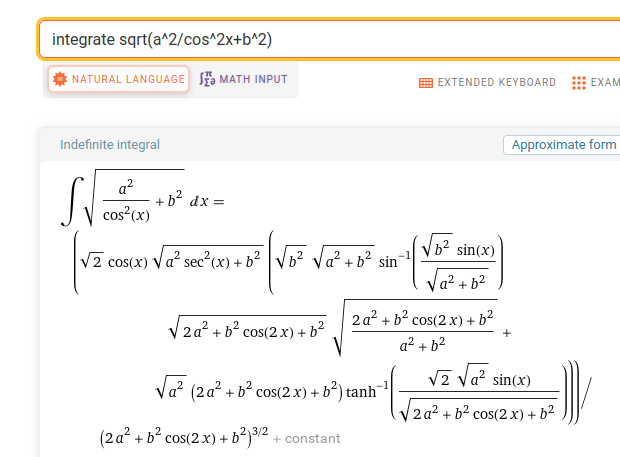
\includegraphics[width=0.7\textwidth]{sol.png}
\end{solution}

\question{A point charge $2Q$ is placed at the center of an air-filled spherical metallic (perfectly conducting) shell, charged with $Q$ and situated in air. The inner and outer radii of the shell are $a$ and $b$ ($a<b$). What is the total charge on the inner and outer surface of the shell, respectively? Find the potential of the shell.}

\begin{solution}
	There is no electric field in the conductor. By Gauss' Law, this means the net enclosed charge $\forall r \in (a,b)$ is 0, meaning a charge of $-2Q$ is concentrated at the inner surface. For the total charge to be $Q$, there is a charge of $3Q$ on the outer surface. Due to Gauss' Law, if there is spherical symmetry, we can treat all the charges to be concentrated at the centre. The potential is then
	$$V = \frac{3kQ}{b}$$
\end{solution}

\question{Prove that the electric potential at an arbitrary point on the $z$-axis produced by the semi-circular line charge of \ref{q} is
	$$V = \frac{\rho_la}{4\varepsilon_0\sqrt{z^2+a^2}}$$
}

\begin{solution}
	\begin{align*}
		V &= \int_{_\frac{\pi}{2}}^{\frac{\pi}{2}} \frac{\rho_lad\phi}{4\pi\varepsilon_0\sqrt{z^2+a^2}} \\
		  &= \frac{\rho_la}{4\varepsilon_0\sqrt{z^2+a^2}}
	\end{align*}
\end{solution}

\question{Determine the electric potential at the center of a non-uniformly charged spherical surface of radius $a$, with $\rho_s(\theta) = \rho_{s,o}\sin(2\theta)$, with $\rho_{s,o}$ a constant and the angle $0 \leq \theta \leq \pi$.}

\begin{solution}
	\begin{align*}
		V &= \int_0^{2\pi} \int_0^\pi \frac{k\rho_{s,o}\sin2\theta a\sin\theta d\theta d\phi}{a} \\
		  &= k\rho_{s,o} \int_0^{2\pi} \int_0^\pi 2\sin^2\theta d(\sin\theta) d\phi \\
		  &= k\rho_{s,o} \int_0^{2\pi} 0d\phi \\
		  &= 0
	\end{align*}
	Or simply, note that for any point on the sphere, its opposite point on the sphere has the opposite charge, hence they all cancel out.
\end{solution}

\question{Find the distribution of the electric scalar potential inside and outside a sphere $R = \alpha$ with volume charge density: $\rho = \rho_0\frac{R}{\alpha}$, where $R$ is the radial coordinate of the spherical coordinate system.}

\begin{solution}
	Charge inside the sphere at radius $r$ is
	\begin{align*}
		Q &= \int_0^{2\pi} \int_0^\pi \int_0^r \rho_0\frac{R}{\alpha} R^2\sin\theta drd\theta d\phi \\
		  &= \int_0^{2\pi} \int_0^\pi \rho_0 \frac{r^4}{4\alpha} \sin\theta d\theta d\phi \\
		  &= \int_0^{2\pi} \rho_0 \frac{r^4}{2\alpha} d\phi \\
		  &= \frac{r^4\rho_0\pi}{\alpha}
	\end{align*}
	Then using Gauss' Law, $\vec{E}$ inside the sphere is
	\begin{align*}
		4\pi r^2 E_r &= \frac{r^4\rho_0\pi}{\alpha\varepsilon_0} \\
		E_r &= \frac{r^2\rho_0}{4\alpha\varepsilon_0}
	\end{align*}
	Ouside of the sphere,
	$$E_r = \frac{\alpha^3\rho_0}{4\varepsilon_0r^2}$$
	And voltage outside the sphere is
	$$V = \frac{\alpha^3\rho_0}{4\varepsilon_0r}$$
	Voltage inside the sphere is
	$$\int_r^\infty Edr = \int_r^\alpha Edr + \int_\alpha^\infty Edr = \frac{\rho_0(\alpha^3-R^3)}{12\varepsilon_0\alpha} + \frac{\rho_0\alpha^2}{4\varepsilon_0} = \frac{\rho_0\alpha^2}{3\varepsilon_0} - \frac{\rho_0R^3}{12\varepsilon_0\alpha}$$
\end{solution}

\question{Find the work done by electric forces in moving a charge $Q = 1\unit{nC}$ from the coordinate origin to the point (1m, 1m, 1m) in the electrostatic field given by $\vec{E}(x,y,z) = (x\hat{a}_x + y^2\hat{a}_y - \hat{a}_z)$ V/m along the straight line.}

\begin{solution}
	\begin{align*}
		\text{Work Done} &= -\int 10^{-9}(x\hat{a}_x + y^2\hat{a}_y - \hat{a}_z)\cdot d\vec{l} \\
				 &= -\int_0^1 10^{-9}(t\hat{a}_x + t^2\hat{a}_y - \hat{a}_z)\cdot(\hat{a}_x + \hat{a}_y + \hat{a}_z) dt \\
				 &= -\int_0^1 10^{-9}(t^2 + t - 1)dt \\
				 &= \frac{1}{6}\unit{nJ}
	\end{align*}
\end{solution}

\question{A finite line charge of length $L$ carrying uniform line charge density $\rho_l$ is coincident with the $x$-axis. In the plane bisecting the line charge ($yz$-plane) determine potential $V$.}

\begin{solution}
	\begin{align*}
		V &= 2\int_0^L \frac{k\rho_l dx}{\sqrt{x^2+y^2+z^2}} \\
		  &= 2k\rho_0\left(\ln\left(\sqrt{\frac{L^2}{4} + y^2 + z^2} + \frac{L}{2}\right) - \ln\sqrt{y^2 + z^2}\right)
	\end{align*}
\end{solution}

\question{Charge $Q$ is distributed over the wall of a circular tube of radius $b$ and height $h$. The tube sits on $xy$-plane with its axis coinciding with $z$-axis. Determine $V$ and $\vec{E}$ along the axis of the tube.}

\begin{solution}
	\begin{align*}
		V(Z) &= \int_0^h \int_0^{2\pi} \frac{k\rho_s bd\phi dz}{\sqrt{(z-Z)^2 + b^2}} \\
		     &= \frac{\rho_s b}{2\varepsilon_0} \int_0^h \frac{dz}{\sqrt{(z-Z)^2 = b^2}} \\
		     &= \frac{\rho_sb}{2\varepsilon_0}\ln\frac{\sqrt{(Z-h)^2 + b^2} - (Z-h)}{\sqrt{Z^2 + b^2} - Z}
	\end{align*}
	Differentiating,
	$$E = \frac{\rho_sb}{2\varepsilon_0}\left(\frac{1}{\sqrt{(z-h)^2+b^2}} - \frac{1}{\sqrt{z^2+b^2}}\right)$$
\end{solution}

\question{Consider the system of two metallic spheres connected by a wire. Assume that $a$ = 5 cm, $b$ = 1 cm, and $d$ = 1 m, as well as that the total charge of the two spheres is $Q = 600 \unit{pC}$. Find the potential of the spheres and the electric field intensities $E_a,E_b$ near the surfaces of the spheres.}

\begin{solution}
	The surface voltages have to be equal, so
	\begin{align*}
		V_a &= V_b \\
		\frac{kQ_a}{a} &= \frac{kQ_b}{b} \\
		\frac{Q_a}{a} &= \frac{Q_b}{b}
	\end{align*}
	Considering the sum of charges,
	$$Q_a = 500\unit{pC}, Q_b = 100\unit{pC}$$
	Substituting, the potentials are then $89.9\unit{V}$. \\
	The fields are then $\frac{4.49}{r^2}$ and $\frac{0.899}{r^2}$ respectively.
\end{solution}
\end{questions}
\end{document}
